
\chapter{Judges and Officials Rules}

\section{Basketball Director}

The Basketball Director is the head organizer and administrator of basketball events.
The Basketball Director is responsible for the logistics and equipment for the basketball competition.
The Basketball Director is in charge of keeping events running on schedule.

\section{Game Referee}

The Game Referee is the head official for a game, whose primary job is to make sure the competitors follow the rules.
The Game Referee makes all final decisions regarding rule infractions.
The Game Referee is responsible for resolving protests.

\newpage
\section{Referee Signals}

\oldrule{10.12}
\textbf{Administrative signals:}

\begin{figure}[h]
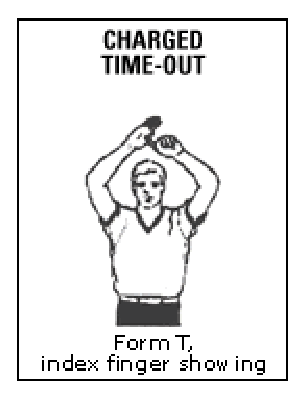
\includegraphics[scale=0.6]{1-a_signal}
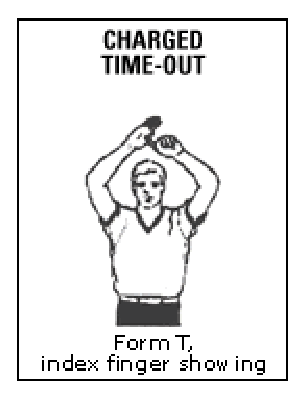
\includegraphics[scale=0.6]{1-b_signal}
\end{figure}

\textbf{Scoring signals:}
\begin{figure}[h]
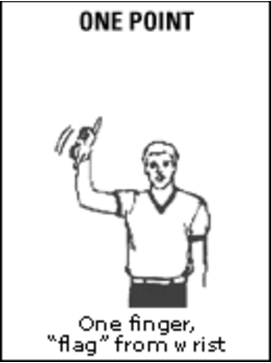
\includegraphics[scale=0.6]{2-a_signal}
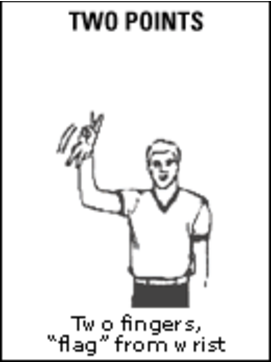
\includegraphics[scale=0.6]{2-b_signal}
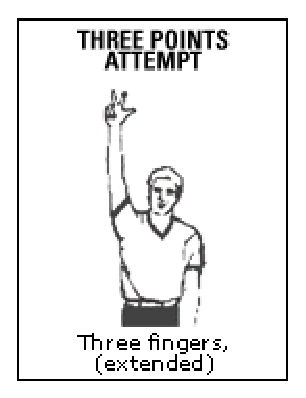
\includegraphics[scale=0.6]{2-c_signal}
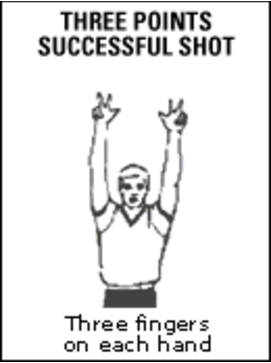
\includegraphics[scale=0.6]{2-d_signal}
\end{figure}

\textbf{Violation signals:}

\begin{figure}[h]

\includegraphics[scale=0.6]{3-a_signal}

\includegraphics[scale=0.6]{3-b_signal}
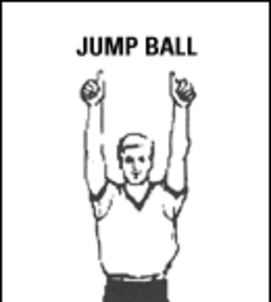
\includegraphics[scale=0.6]{3-c_signal}
\end{figure}
